\documentclass{article}
\usepackage{graphicx} % Required for inserting images
\usepackage{biblatex}
\usepackage{float}
\addbibresource{references.bib}

\title{Phase Conditioned Sparsity for Automated Program Repair}

\date{June 2026}

\begin{document}

\maketitle

\section{Overview}

Software bugs are costly. Beyond the developer effort spent resolving them, they can trigger failures with substantial financial consequences~\cite{BentonFCC2024, BusinessInsider2024, ZahnEtAl2024}. Resolving such bugs is therefore a challenge in software development~\cite{Zouz2020}, and a time-consuming one: developers are estimated to spend roughly half of their time on debugging and bug resolution~\cite{Britton2013}. This process is cognitively demanding, as it requires a deep understanding of the codebase~\cite{ByungDo1998,Hu2024}. To assist developers with this activity, automated program repair (APR) has been proposed~\cite{Gazzola2019}. Traditionally, these systems have relied on information retrieval and template-based solutions. However, these approaches are often rigid, making it difficult to extrapolate them to unseen scenarios. Large language models (LLMs) and LLM-based systems offer great promise in this regard: because these massive models are trained on vast datasets, they possess stronger generalization capabilities. Methods like Agentless~\cite{Xia2025} and SWE-agent~\cite{Yang2024sweagent} demonstrate a remarkable aptitude for resolving issues compared to classical APR methods.

However, the massive scale of these models makes them expensive to operate. This cost is multifaceted: computational (requiring extensive arithmetic operations), monetary (demanding high-end computing infrastructure), and environmental (correlating increased compute with higher emissions). It is well established that LLMs are over-parameterized: not every neuron contributes equally to a given computation, and ablating a subset can incur only minimal performance degradation~\cite{Voita2019, Sandovalsegura2026identifying, Dong2024promptprompted}. Moreover, the set of components that matter is often \emph{input-dependent}, a phenomenon known as contextual sparsity~\cite{Liu2023dejavu}, and prior work has localized specific skills or functions to identifiable groups of neurons~\cite{Wang2022skillneurons}. Separately, automated bug resolution follows a structured workflow: localizing the bug, reproducing it, issuing a patch, and finally running tests to verify the fix and check for regressions. In light of these two observations, we hypothesize that distinct regions of the network could be activated during the phases of the APR process. A pictorial representation of this hypothesis is illustrated in Figure~\ref{fig:main_hypothesis}. If this holds, the phase becomes a conditioning signal for sparsity: because an APR agent always knows which phase it is currently executing, we could selectively activate (or prune) only the relevant regions per phase, reducing the floating-point operations and latency of each step without sacrificing repair accuracy.


\begin{figure}[H]
    \centering
    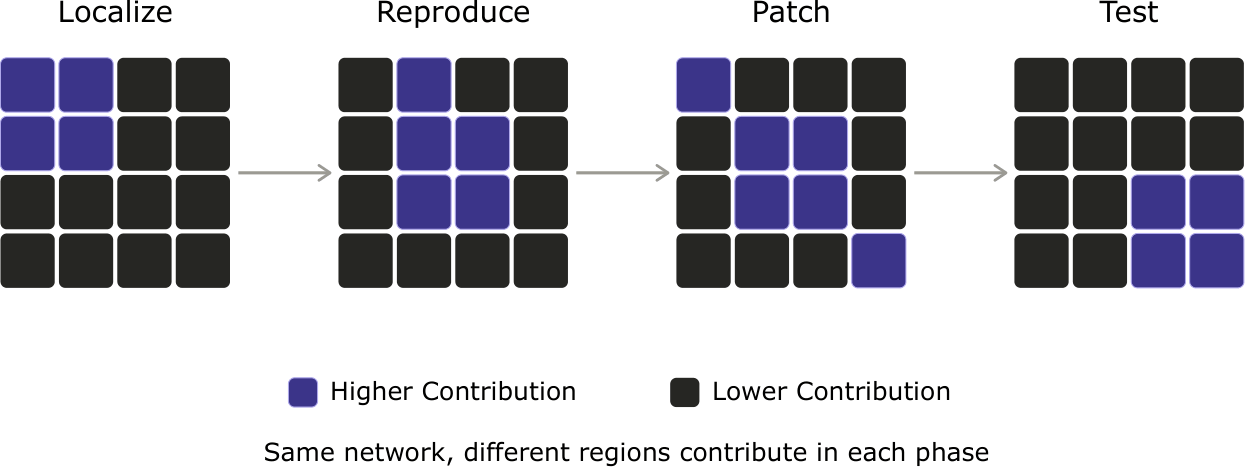
\includegraphics[width=\linewidth]{figures/apr_phase_neuron_activation_grid-1.png}
    \caption{Main hypothesis that states that regions of the network are conditioned on the phase of automated program repair.}
    \label{fig:main_hypothesis}
\end{figure}

\section{Research Questions}
We organize the investigation around three research questions that move from existence to exploitation:
\begin{itemize}
    \item \textbf{RQ1 (Existence).} Are neuron and attention-head activations separable by APR phase? That is, given the hidden activations produced while the model performs localization, reproduction, patching, or test/verification, can the phase be recovered from the activation pattern alone?
    \item \textbf{RQ2 (Structure).} If such separation exists, is it consistent and interpretable? How much do the active sets overlap across phases (e.g., measured via Jaccard similarity), are the same regions reused across different bugs and projects, and are the implicated components causally necessary for their phase?
    \item \textbf{RQ3 (Compute Efficiency).} Can phase-conditioned sparsity be exploited to reduce computational cost, floating-point operations, latency, or memory, with sacrificing too much performance?
\end{itemize}

\section{Approach}
The following is a tentative methodology which can be refined as the project progresses.

\paragraph{Defining a phase.} We take a \emph{phase} to be an agent step (or prompt role) within an established APR scaffold such as Agentless~\cite{Xia2025} or SWE-agent~\cite{Yang2024sweagent}: bug localization, reproduction, patch generation, and test/verification.The main goal is to investigate if there exist \emph{consistent, reusable} sub-circuits within a single model serving all phases. A minimal ReACT-based agent can also be implemented, if needed.

\paragraph{Models.} Neuron-level inspection requires access to model weights, so we focus on open-weights code LLMs (e.g., Qwen2.5-Coder or DeepSeek-Coder).

\paragraph{Data and harness.} SWE-bench (Verified or Lite), Defects4J.

\paragraph{Units and attribution.} The units of analysis are MLP neurons and attention heads, taken per layer. To attribute components to phases, we plan to combine (i) mean/peak activation statistics per phase, (ii) lightweight probing classifiers that predict the phase from activations, (iii) activation-overlap metrics across phases, and (iv) causal ablation to test whether the implicated components are necessary for a given phase. Such methods have been partially covered in the work of~\cite{Sandovalsegura2026identifying}.

\section{Feasibility and Resources}
Because the study targets open-weights models and reuses existing scaffolds and benchmarks, it should be tractable. Access to GPUs is also available.

\section{Logistics and Collaboration}
\begin{itemize}
    \item \textbf{Time commitment:} $6$ months. Number of hours is up to the candidate.
    \item \textbf{Mode:} Remote.
    \item \textbf{Target venue:} To be determined.
    \item \textbf{Authorship:} Ideally, we want the candidate to be the first author. However, that will depend later on their contribution.
\end{itemize}

\section{Minimum Requirements}
An ideal candidate should meet the following minimum requirements:
\begin{itemize}
    \item Interest in conducting research. This includes all aspects of the process from reading literature, to implementation, running experiments, to writing. Of course, the candidate will not be in charge of carrying out all of these activities end-to-end. Rather, they will play a role in every step.
    \item Be relatively comfortable with reading CS-related scientific literature.
    \item A decent understanding of deep learning.
    \item Basic conceptual understanding of the Transformer architecture. Not necessarily those with newer architectural tweaks. A basic understanding of the original architecture proposed by Vaswani et al.\ is enough.
    \item Good Python skills.
\end{itemize}

\section{Nice to Have}
The following are qualifications that are nice-to-have, but can definitely be acquired throughout the project:

\begin{itemize}
    \item Knowledge of recent literature on computationally efficient language models. This includes (un)-structured pruning, sparse neural networks and input compression. This also includes familiarity with concepts related to such subfield such as measurement metrics like number of floating-point operations, throughput, wall-clock time, and so on.
    \item Implemented a decoder-only Transformer model in Pytorch, or played around with an implementation (e.g., using huggingface's transformers library).
\end{itemize}


\printbibliography

\end{document}
